\begin{exercise}
1.判断下列集合的基数是 $\aleph_0, \aleph$ ,还是 $2^{\aleph}$ ,并说明理由:
(1)所有 $n$ 维开矩体*构成的集合 $\mathscr{R}$ ;${ }^{\dagger}$
(2)所有以有理点(即坐标皆为有理数的点)为顶点的 $n$ 维开矩体构成的集合 $\mathscr{Q}$ ;
\end{exercise}
(1)
\[
\#\mathscr{R}=(\#\mathbb{R})^{n}=\aleph
\]
(2)
\[
\#\mathscr{Q}\leq \underbrace{ \mathbb{Q}^{n}\times\dots \times \mathbb{Q}^{n} }_{ n \text{ times} }=\mathbb{Q}^{n^{2}}=\aleph_0
\]
\begin{exercise}
2.是否存在集合族 $\Gamma$ ,使得对任意集合 $B$ ,都存在 $A \in \Gamma$ ,使得 $A \sim B$ ?
\end{exercise}
I don't understand.

\begin{exercise}
3.设 $a, b \in \mathbb{R}^2 \backslash \mathbb{Q}^2$ 且 $a \neq b$ .证明: $\mathbb{R}^2$ 中存在经过 $a$ 和 $b$ 两点且不含有理点的圆周.
\end{exercise}
\begin{proof}
假设任意经过 $a,b$ 两点的圆周都包含有理点,考虑 $a,b$ 的中垂线 $l$,这是一条直线,上面全部点的势为 $\aleph$. 取任意 $c\in l$ 为圆心,作过 $a,b$ 的圆,可以找到一个不同于 $a,b$ 的点 $p_{c}\in \mathbb{Q}^{2}$,我们有如下自然映射
\[
\varphi:l \to \mathbb{Q}^{2}\qquad c\mapsto p_{c}
\]
这显然是个单射,因为任意两个不完全重合的圆至多有两个交点,而刚才取的圆都交于 $a,b$,故 $c_1\neq c_2\Rightarrow p_{c_1}\neq p_{c_2}$. 因此
\[
\#l=\#\varphi(l)\leq \#\mathbb{Q}^{2}=\aleph_0
\]
矛盾!
\end{proof}

\begin{exercise}
4.设 $A \subset \mathbb{R}^n$ 是可数集.证明:存在 $x \in \mathbb{R}^n$ ,使得 $A \cap(A+x)=\varnothing$ .
\end{exercise}
\begin{proof}
Assume, for contradiction, that for any $x\in \mathbb{R}^{n}$, there exists $y_{x}\in \mathbb{R}^{n}$ such that
\[
y_{x}\in A\cap(A+x)
\]
That is
\[
y_{x}\in A\text{ and }y_{x}-x\in A
\]
Construct the following map
\[
\varphi:\mathbb{R}^{n}\hookrightarrow A\times A\qquad x\longmapsto(y_{x},y_{x}-x)
\]
which is 1-1, sisnce $(y_{x_1},y_{x_1}-x_1)=(y_{x_2},y_{x_2}-x_2)\Rightarrow y_{x_1}=y_{x_2},x_1=x_2$. Thus
\[
\#\mathbb{R}^{n}=\#\varphi(\mathbb{R}^{n})\leq \#(A\times A)=(\#A)^{2}=\aleph_0
\]
which is a contradiction.
\end{proof}

\begin{exercise}
5.教材第一章习题第 42 题(1)(2).
\begin{figure}[H]
\centering
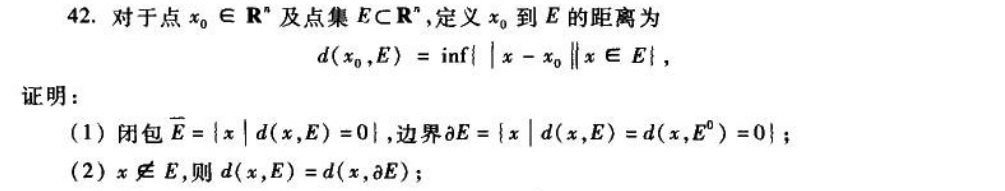
\includegraphics[width=\textwidth]{hw3-20250323.png}
% \caption{}
\label{}
\end{figure}
\end{exercise}
\begin{proof}
(1)
If $d(x,E)=0$ then $\inf \{ \lvert x-x' \rvert:x'\in E \}=0$ which means that $x$ is a limit point of $E$. By definition,
\[
\overline{E}=\{ x:d(x,E)=0 \}
\]
Errata: $\partial E\neq \{ x:d(x,E)=d(x,{\mathring E})=0 \}$.
\[
\partial E=\overline{E}\setminus {\mathring E}
\]
(2)
For any $x\not\in E$, check that
\[
\inf \{ \lvert x-y \rvert :y\in E \}=\inf \{ \lvert x-z \rvert :z\in \partial E=\overline{E}\setminus{\mathring E}  \}
\]
Denote that
\[
r=\inf \{ \lvert x-y \rvert :y\in E \},\quad s=\inf \{ \lvert x-z \rvert :z\in \partial E=\overline{E}\setminus{\mathring E}  \}
\]
Then $\forall\epsilon>0,\exists z\in \partial E$ s.t.
\[
\lvert x-z \rvert \leq s+\epsilon
\]
Pick $\widehat{z}\in B_{z}(\epsilon)\cap E$, then
\[
\lvert x-\widehat{z} \rvert \leq \lvert x-z \rvert +\lvert z-\widehat{z} \rvert \leq s+2\epsilon
\]
Thus
\[
\inf_{y\in E}\lvert x-y \rvert \leq s+2\epsilon
\]
Since $\epsilon$ is arbitrary, we have
\[
r\leq s
\]
WLOG, assume that $E$ is bounded (otherwise we replace $E$ by $E\cap \{ y:\lvert y-x \rvert\leq r+1 \}$)

Pick $x_n$ in each $\left\{  y:\lvert y-x \rvert\leq r+\frac{1}{n}  \right\}$ for $n\in \mathbb{N}$. Since $\overline{E}$ is closed and bounded, thus compact, thus sequentially compact. Then $\{ x_n \}\to \widehat{x}$ for some $\widehat{x}\in \overline{E}$. Obviously, $\widehat{x}\in \partial E$. We have
\[
\inf_{y\in E}\lvert x-y \rvert =\lvert x-\widehat{x} \rvert \geq \inf_{z\in \partial E}\lvert x-z \rvert
\]
That is
\[
r\geq s
\]
Hence
\[
r=s
\]
\end{proof}

\begin{exercise}
6.教材第一章习题第 43 题.
\begin{figure}[H]
\centering
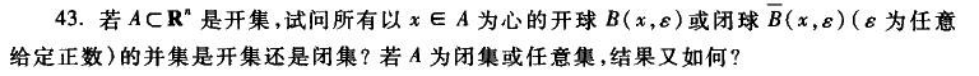
\includegraphics[width=\textwidth]{hw3-2025032323.png}
% \caption{}
\label{}
\end{figure}
\end{exercise}
Since open set remains open under any intersection. That is, for any set $A$, $\bigcup_{x\in A}B(x,\epsilon)$ is open.

Now we consider $\bigcup_{x\in A}\overline{B}(x,\epsilon)$.

If $A$ is open, pick any $y\in \bigcup_{x\in A}\overline{B}(x,\epsilon)$, then $y\in \overline{B}(x,\epsilon)$ for some $x\in A$. There exists $z=\theta x+(1-\theta) y\in A$ for some $\theta\in(0,1)$, then $y\in \overline{B}(z,\epsilon)\subset \bigcup_{x\in A}\overline{B}(x,\epsilon)$. Thus $y$ is an interior point of $\bigcup_{x\in A}\overline{B}(x,\epsilon)$. Hence $\bigcup_{x\in A}\overline{B}(x,\epsilon)$ is open.

If $A$ is closed. Check that $E=\bigcap_{x\in A}\{ y:\lvert y-x \rvert>\epsilon \}$ is open.

Pick $z\in E$, then $\lvert z-x \rvert>\epsilon,\forall x\in A$. Pick $x_n$ in each $\left\{  x:\lvert x-d(x,A) \rvert<\frac{1}{n}  \right\}$, then $\{ x_n \}\to \widehat{x}$ for some $\widehat{x}\in A$, thus $\lvert z-\widehat{x} \rvert=\inf_{x\in A}\lvert z-x \rvert$. Let $\delta=\frac{1}{2}(\lvert x-\widehat{x} \rvert-\epsilon)$, then $B_{\delta}(z)\subset E$. $z$ is an interior point of $E$. Hence $E$ is open.

If $A=[0,1)^{n}$ then $\bigcup_{x\in A}\overline{B}(x,\epsilon)$ is neither open nor closed.

\begin{exercise}
7.若 $A, B$ 都是 $\mathbb{R}^n$ 的闭集,是否一定存在 $x_0 \in A, y_0 \in B$ ,使得 $d\left(x_0, y_0\right)=d(A, B)$ ?予以证明或举出反例.
\end{exercise}
不妨设 $A,B$ 为有界闭集,则 $A,B$ 为紧集,故列紧. 由 $d(A,B)$ 的定义可知,存在 $\{ (x_n, y_n) \}\in A\times B$ 使得 $d(A,B)=\lim_{ n \to \infty }d(x_n,y_n)=d(x_0,y_0)$,其中 $(x_0, y_0)\in A\times B$.

\begin{exercise}
8.试构造下列各函数(列).
(1)设 $A, B$ 是 $\mathbb{R}^n$ 中互不相交的非空闭集.试作 $\mathbb{R}^n$ 上的连续函数 $f$ ,使得
(i) $0 \leqslant f(x) \leqslant 1, \forall x \in \mathbb{R}^n$ ;
(ii)$f(x)=0, \forall x \in A$ ;
(iii)$f(x)=1, \forall x \in B$ .
(2)设 $A, B \subset \mathbb{R}^n$ ,且满足 $\bar{A} \cap B=\bar{B} \cap A=\varnothing$ .试作 $\mathbb{R}^n$ 上的连续函数 $f$ ,使得
(i)$f(x)<0, \forall x \in A$ ;
(ii)$f(x)>0, \forall x \in B$ .
(3)设 $F$ 是 $\mathbb{R}^n$ 的闭集.试作 $\mathbb{R}^n$ 上的连续函数序列 $\left\{f_k\right\}$ ,使得 $\lim _{k \rightarrow \infty} f_k(x)=\chi_F(x)$ , $\forall x \in \mathbb{R}^n$ .
(4)设 $G$ 是 $\mathbb{R}^n$ 的开集.试作 $\mathbb{R}^n$ 上的连续函数序列 $\left\{f_k\right\}$ ,使得 $\lim _{k \rightarrow \infty} f_k(x)=\chi_G(x)$ , $\forall x \in \mathbb{R}^n$.
\end{exercise}
(1)
\[
f(x)=\frac{d(x,A)}{d(x,A)+d(x,B)}
\]
(2)
\[
f(x)=d(x,A)-d(x,B)
\]
(3)
\[
f_k(x)=\frac{1}{1+kd(x,F)}
\]
(4)
\[
f_k(x)=\frac{kd(x,G^{c})}{1+kd(x,G^{c})}
\]
\begin{exercise}
9.教材第一章习题第 44 题.
\begin{figure}[H]
\centering
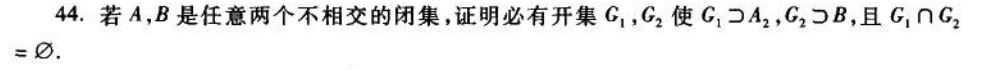
\includegraphics[width=\textwidth]{hw3-2025032400.png}
% \caption{}
\label{}
\end{figure}
\end{exercise}
Note that all the sets must lies in a metric space. And the property $A,B$ satisfy is called Normal separation property.

Let
\[
F_1\subseteq \mathcal{O}_{1}\coloneqq \{ x:d(x,F_1)<d(x,F_2) \}
\]
\[
F_2\subseteq \mathcal{O}_{2}\coloneqq \{ x:d(x,F_1)>d(x,F_2) \}
\]
Then $\mathcal{O}_{1}\cap \mathcal{O}_{2}=\varnothing$.

\begin{exercise}
10.教材第一章习题第 45 题.
\begin{figure}[H]
\centering
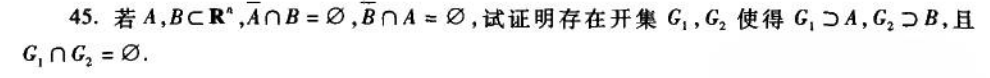
\includegraphics[width=\textwidth]{1-hw3-2025032400.png}
% \caption{}
\label{}
\end{figure}
\end{exercise}
证不出来

\begin{exercise}
11.教材第一章习题第 46 题.
\begin{figure}[H]
\centering
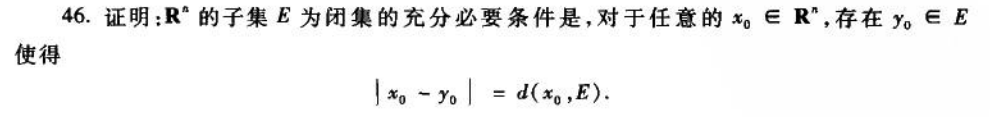
\includegraphics[width=\textwidth]{2-hw3-2025032400.png}
% \caption{}
\label{}
\end{figure}
\end{exercise}
必要性显然,考虑充分性,假设 $E$ 不是闭集,则存在一个包含在 $E$ 中的极限点 $x_0$,于是存在 $y_0\in E$ 使得
\[
\lvert x_0-y_0 \rvert =d(x_0,E)=0
\]
于是 $x_0=y_0\in E$,矛盾!

\begin{exercise}
12.教材第一章习题第 48 题.
\begin{figure}[H]
\centering
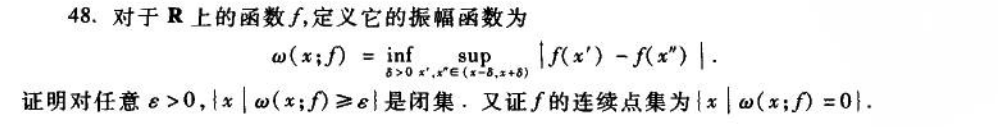
\includegraphics[width=\textwidth]{3-hw3-2025032400.png}
% \caption{}
\label{}
\end{figure}
\end{exercise}
下面证明 $\{ x:\omega(x;f)<\epsilon \}$ 是开集. 任意给定 $x\in \{x: \omega(x;f)<\epsilon \}$,记
\[
r=\inf_{\delta>0}\underbrace{ \sup_{x',x''\in(x-\delta,x+\delta)} \lvert f(x')-f(x'') \rvert }_{ \eqqcolon A(x,\delta) } <\epsilon
\]
对于任意给定的 $\epsilon'\in\left( 0,\frac{\epsilon-r}{2} \right)$,存在 $\widehat{\delta}>0$,使得
\[
A(x,\widehat{\delta})\geq r+\epsilon'<\epsilon
\]
那么对于任意的 $y\in B_{\widehat{\delta}/2 }(x)$,有
\[
A\left( y,\widehat{\delta}/2 \right)\leq A(x,\widehat{\delta})<\frac{\epsilon+r}{2}<\epsilon
\]
因此
\[
\inf_{\delta>0}\sup_{x',x''\in(y-\delta,y+\delta)}\lvert f(x')-f(x'') \rvert <\epsilon
\]
故 $B_{\widehat{\delta}/2}(x)\subset \{ x:\omega(x;f)<\epsilon \}$. 得证!

再用 $C$ 表示 $f$ 的连续点集,显然 $C\subseteq \{ x:\omega(x;f)=0 \}$. 另一方面,对于任意 $x\in \{ x:\omega(x;f)=0 \}$,
\[
\inf_{\delta>0}\sup_{x',x''\in(x-\delta,x+\delta)}\lvert f(x')-f(x'') \rvert =0
\]
也就是说,对于任意 $\epsilon>0$,存在 $\delta>0$,使得
\[
\sup_{x',x''\in(x-\delta,x+\delta)}\lvert f(x')-f(x'') \rvert  <\epsilon
\]
这就是 $f$ 在 $x$ 处连续的定义.
